\section{Redes de Hopfield}

\begin{frame}{Redes de Hopfield}%
  \justifying%
  Uma rede de Hopfield é uma rede que armazena padrões de tal forma que quando um padrão novo é mostrado para a rede, ela responde devolvendo o padrão que ela tem armazenado mais próximo ao novo padrão.

  Hopfield é uma rede determinística.
\end{frame}

\subsection{Definições}
\begin{frame}{Quais os elementos básicos para Hopfield?}%
  \justifying%
  Vamos considerar que cada uma das \textbf{unidades} da rede é denominada por $\mathrm{x}_{i}$, onde $i = 1, \dots, N$, para uma rede com $N$ unidades.
  
  Em Hopfield, cada $\mathrm{x}_{i}$ pode assumir um dos valores $x_{i} \in \{0, 1\}$. Rede binária!

  Se $x_{i} = 0$, a unidade $i$ desativada; se $x_{i} = 1$, unidade $i$ ativada.
\end{frame}

\begin{frame}{Quais os elementos básicos para Hopfield?}%
  \justifying%
  Os \textbf{pesos} chamaremos de $\omega$.
  
  Na rede de Hopfield os pesos são simétricos, isto é, $\omega_{ij} = \omega_{ji}$ (conexão entre as unidades $i$ e $j$).
  
\end{frame}

\subsection{Esquema}
\begin{frame}{Rede de Hopfield diagrama}
  \begin{figure}[h]{}%
    \label{fig:hopfield}%
    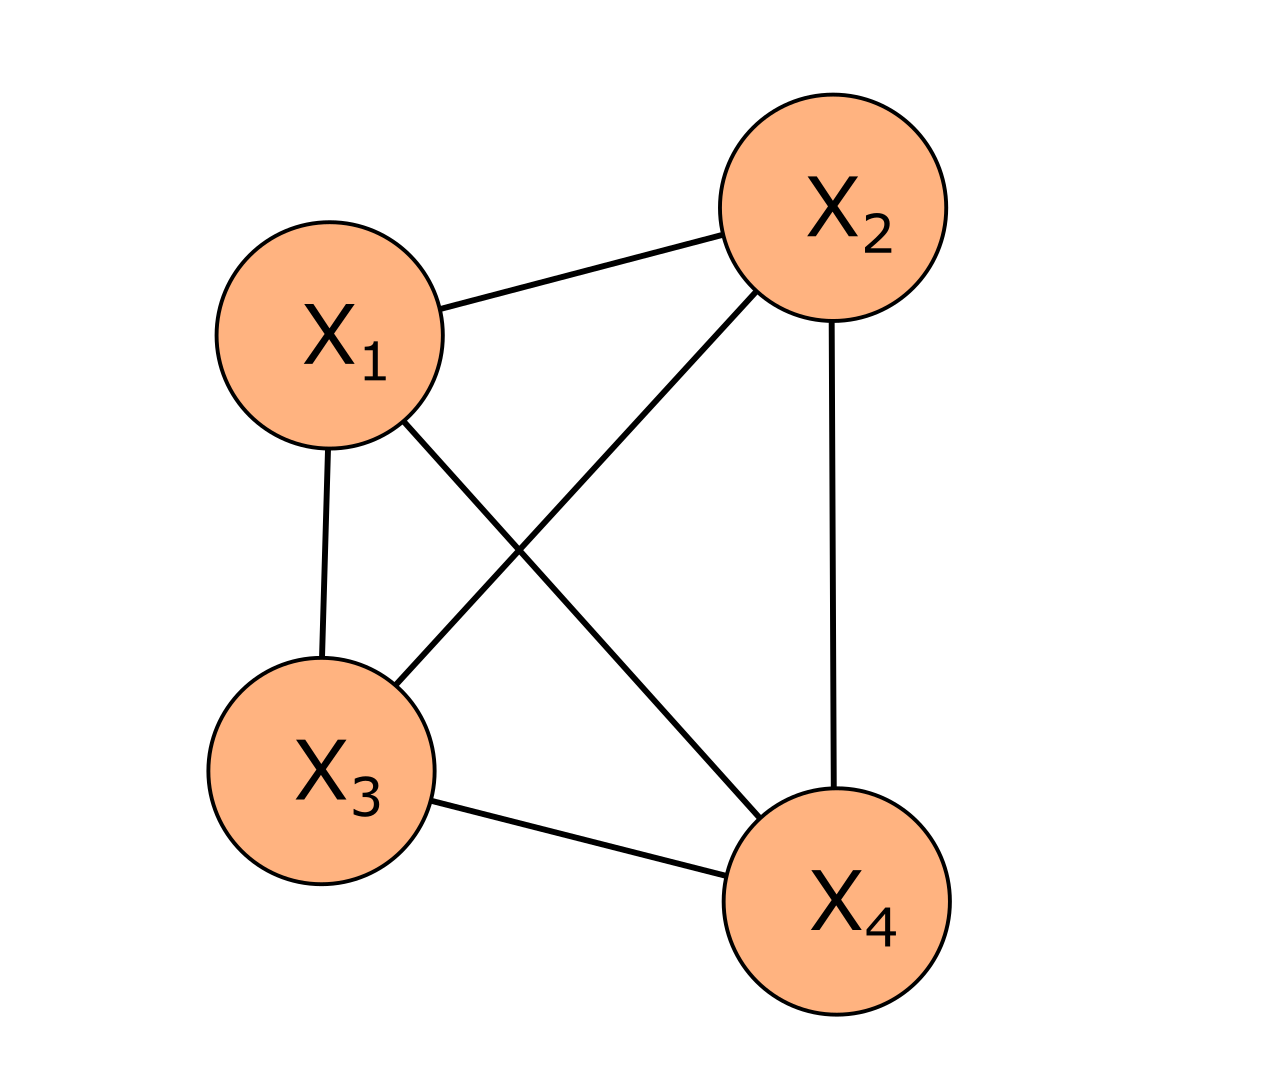
\includegraphics[scale=0.5]{images/hopfield.png}
    \caption{Distribuição dos neurônios de uma rede de Hopfield com 4 unidades.}
  \end{figure}
\end{frame}

\begin{frame}{Rede de Hopfield diagrama}
  \begin{figure}[h]{}%
    \label{fig:hopfield-full}%
    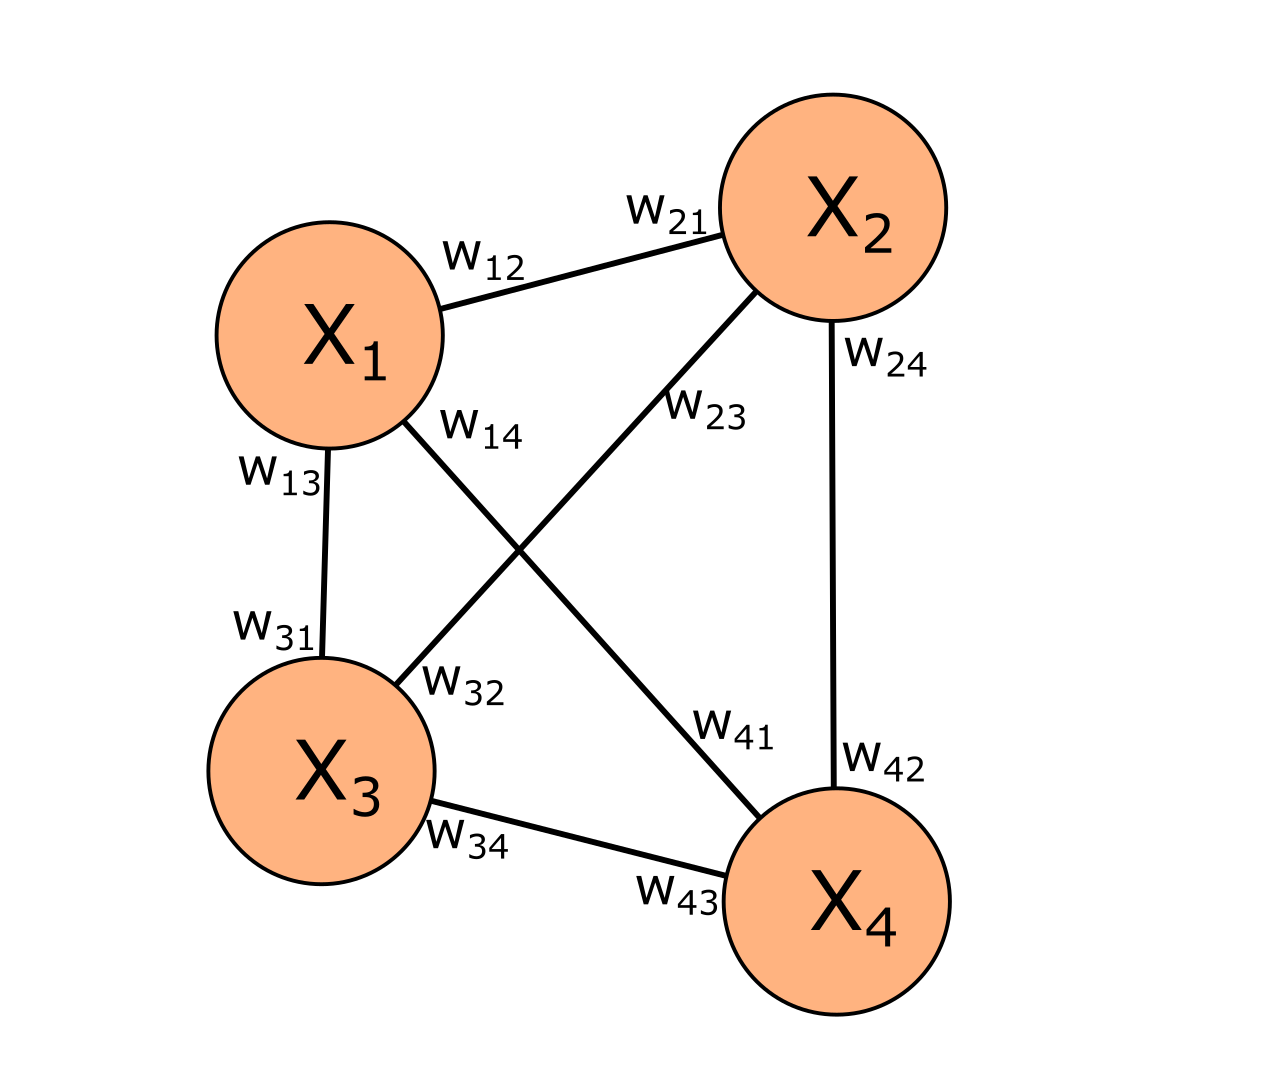
\includegraphics[scale=0.5]{images/hopfield_full.png}
    \caption{Identificação das conexões de uma rede de Hopfield com 4 unidades.}
  \end{figure}
\end{frame}

\subsection{Funcionamento}
\begin{frame}{}
\end{frame}
